\documentclass[1p]{elsarticle_modified}
%\bibliographystyle{elsarticle-num}

%\usepackage[colorlinks]{hyperref}
%\usepackage{abbrmath_seonhwa} %\Abb, \Ascr, \Acal ,\Abf, \Afrak
\usepackage{amsfonts}
\usepackage{amssymb}
\usepackage{amsmath}
\usepackage{amsthm}
\usepackage{scalefnt}
\usepackage{amsbsy}
\usepackage{kotex}
\usepackage{caption}
\usepackage{subfig}
\usepackage{color}
\usepackage{graphicx}
\usepackage{xcolor} %% white, black, red, green, blue, cyan, magenta, yellow
\usepackage{float}
\usepackage{setspace}
\usepackage{hyperref}

\usepackage{tikz}
\usetikzlibrary{arrows}

\usepackage{multirow}
\usepackage{array} % fixed length table
\usepackage{hhline}

%%%%%%%%%%%%%%%%%%%%%
\makeatletter
\renewcommand*\env@matrix[1][\arraystretch]{%
	\edef\arraystretch{#1}%
	\hskip -\arraycolsep
	\let\@ifnextchar\new@ifnextchar
	\array{*\c@MaxMatrixCols c}}
\makeatother %https://tex.stackexchange.com/questions/14071/how-can-i-increase-the-line-spacing-in-a-matrix
%%%%%%%%%%%%%%%

\usepackage[normalem]{ulem}

\newcommand{\msout}[1]{\ifmmode\text{\sout{\ensuremath{#1}}}\else\sout{#1}\fi}
%SOURCE: \msout is \stkout macro in https://tex.stackexchange.com/questions/20609/strikeout-in-math-mode

\newcommand{\cancel}[1]{
	\ifmmode
	{\color{red}\msout{#1}}
	\else
	{\color{red}\sout{#1}}
	\fi
}

\newcommand{\add}[1]{
	{\color{blue}\uwave{#1}}
}

\newcommand{\replace}[2]{
	\ifmmode
	{\color{red}\msout{#1}}{\color{blue}\uwave{#2}}
	\else
	{\color{red}\sout{#1}}{\color{blue}\uwave{#2}}
	\fi
}

\newcommand{\Sol}{\mathcal{S}} %segment
\newcommand{\D}{D} %diagram
\newcommand{\A}{\mathcal{A}} %arc


%%%%%%%%%%%%%%%%%%%%%%%%%%%%%5 test

\def\sl{\operatorname{\textup{SL}}(2,\Cbb)}
\def\psl{\operatorname{\textup{PSL}}(2,\Cbb)}
\def\quan{\mkern 1mu \triangleright \mkern 1mu}

\theoremstyle{definition}
\newtheorem{thm}{Theorem}[section]
\newtheorem{prop}[thm]{Proposition}
\newtheorem{lem}[thm]{Lemma}
\newtheorem{ques}[thm]{Question}
\newtheorem{cor}[thm]{Corollary}
\newtheorem{defn}[thm]{Definition}
\newtheorem{exam}[thm]{Example}
\newtheorem{rmk}[thm]{Remark}
\newtheorem{alg}[thm]{Algorithm}

\newcommand{\I}{\sqrt{-1}}
\begin{document}

%\begin{frontmatter}
%
%\title{Boundary parabolic representations of knots up to 8 crossings}
%
%%% Group authors per affiliation:
%\author{Yunhi Cho} 
%\address{Department of Mathematics, University of Seoul, Seoul, Korea}
%\ead{yhcho@uos.ac.kr}
%
%
%\author{Seonhwa Kim} %\fnref{s_kim}}
%\address{Center for Geometry and Physics, Institute for Basic Science, Pohang, 37673, Korea}
%\ead{ryeona17@ibs.re.kr}
%
%\author{Hyuk Kim}
%\address{Department of Mathematical Sciences, Seoul National University, Seoul 08826, Korea}
%\ead{hyukkim@snu.ac.kr}
%
%\author{Seokbeom Yoon}
%\address{Department of Mathematical Sciences, Seoul National University, Seoul, 08826,  Korea}
%\ead{sbyoon15@snu.ac.kr}
%
%\begin{abstract}
%We find all boundary parabolic representation of knots up to 8 crossings.
%
%\end{abstract}
%\begin{keyword}
%    \MSC[2010] 57M25 
%\end{keyword}
%
%\end{frontmatter}

%\linenumbers
%\tableofcontents
%
\newcommand\colored[1]{\textcolor{white}{\rule[-0.35ex]{0.8em}{1.4ex}}\kern-0.8em\color{red} #1}%
%\newcommand\colored[1]{\textcolor{white}{ #1}\kern-2.17ex	\textcolor{white}{ #1}\kern-1.81ex	\textcolor{white}{ #1}\kern-2.15ex\color{red}#1	}

{\Large $\underline{12a_{0095}~(K12a_{0095})}$}

\setlength{\tabcolsep}{10pt}
\renewcommand{\arraystretch}{1.6}
\vspace{1cm}\begin{tabular}{m{100pt}>{\centering\arraybackslash}m{274pt}}
\multirow{5}{120pt}{
	\centering
	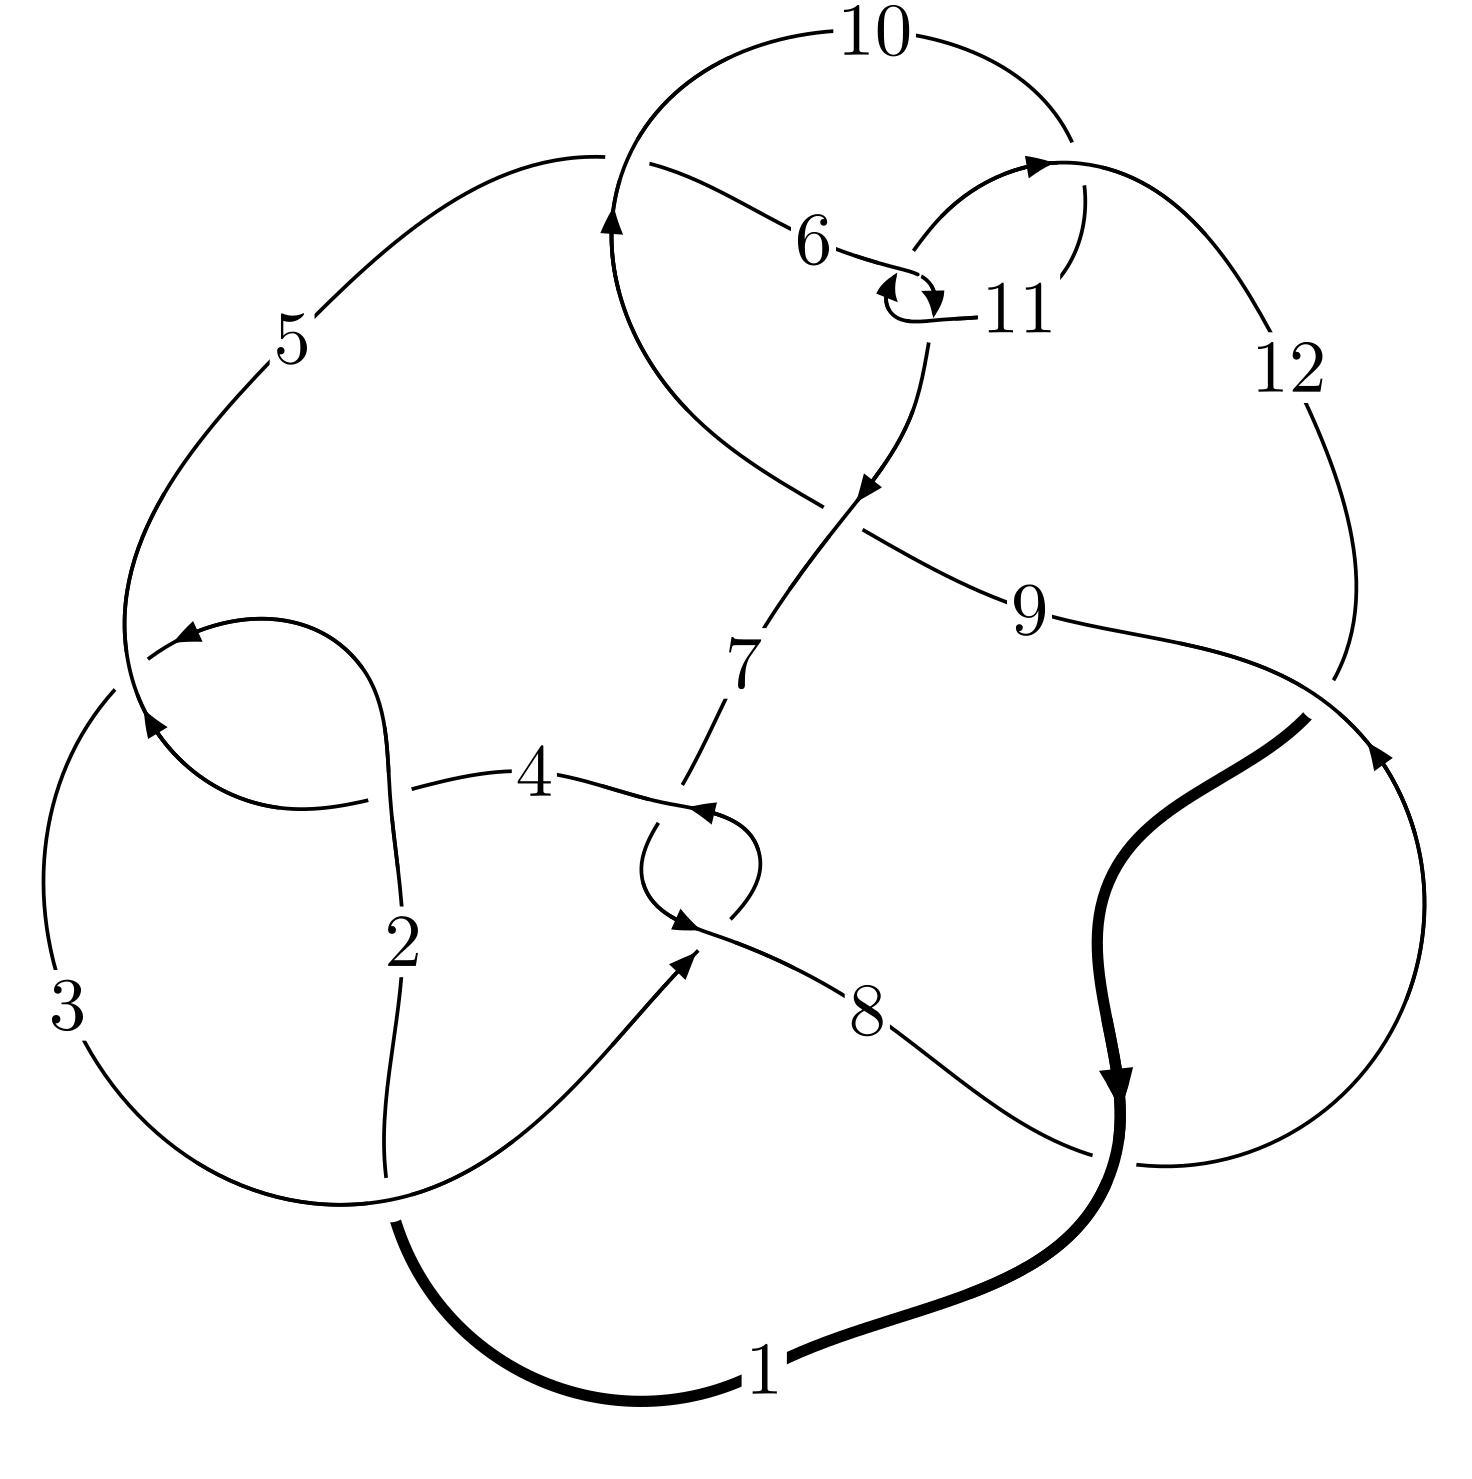
\includegraphics[width=112pt]{../../../GIT/diagram.site/Diagrams/png/896_12a_0095.png}\\
\ \ \ A knot diagram\footnotemark}&
\allowdisplaybreaks
\textbf{Linearized knot diagam} \\
\cline{2-2}
 &
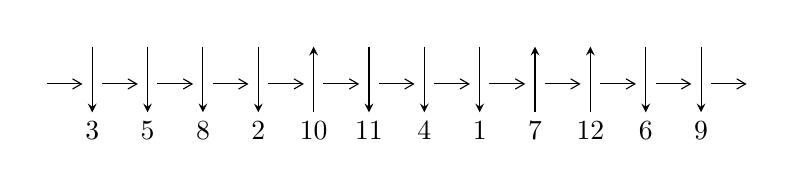
\begin{tikzpicture}[x=20pt, y=17pt]
	% nodes
	\node (C0) at (0, 0) {};
	\node (C1) at (1, 0) {};
	\node (C1U) at (1, +1) {};
	\node (C1D) at (1, -1) {3};

	\node (C2) at (2, 0) {};
	\node (C2U) at (2, +1) {};
	\node (C2D) at (2, -1) {5};

	\node (C3) at (3, 0) {};
	\node (C3U) at (3, +1) {};
	\node (C3D) at (3, -1) {8};

	\node (C4) at (4, 0) {};
	\node (C4U) at (4, +1) {};
	\node (C4D) at (4, -1) {2};

	\node (C5) at (5, 0) {};
	\node (C5U) at (5, +1) {};
	\node (C5D) at (5, -1) {10};

	\node (C6) at (6, 0) {};
	\node (C6U) at (6, +1) {};
	\node (C6D) at (6, -1) {11};

	\node (C7) at (7, 0) {};
	\node (C7U) at (7, +1) {};
	\node (C7D) at (7, -1) {4};

	\node (C8) at (8, 0) {};
	\node (C8U) at (8, +1) {};
	\node (C8D) at (8, -1) {1};

	\node (C9) at (9, 0) {};
	\node (C9U) at (9, +1) {};
	\node (C9D) at (9, -1) {7};

	\node (C10) at (10, 0) {};
	\node (C10U) at (10, +1) {};
	\node (C10D) at (10, -1) {12};

	\node (C11) at (11, 0) {};
	\node (C11U) at (11, +1) {};
	\node (C11D) at (11, -1) {6};

	\node (C12) at (12, 0) {};
	\node (C12U) at (12, +1) {};
	\node (C12D) at (12, -1) {9};
	\node (C13) at (13, 0) {};

	% arrows
	\draw[->,>={angle 60}]
	(C0) edge (C1) (C1) edge (C2) (C2) edge (C3) (C3) edge (C4) (C4) edge (C5) (C5) edge (C6) (C6) edge (C7) (C7) edge (C8) (C8) edge (C9) (C9) edge (C10) (C10) edge (C11) (C11) edge (C12) (C12) edge (C13) ;	\draw[->,>=stealth]
	(C1U) edge (C1D) (C2U) edge (C2D) (C3U) edge (C3D) (C4U) edge (C4D) (C5D) edge (C5U) (C6U) edge (C6D) (C7U) edge (C7D) (C8U) edge (C8D) (C9D) edge (C9U) (C10D) edge (C10U) (C11U) edge (C11D) (C12U) edge (C12D) ;
	\end{tikzpicture} \\
\hhline{~~} \\& 
\textbf{Solving Sequence} \\ \cline{2-2} 
 &
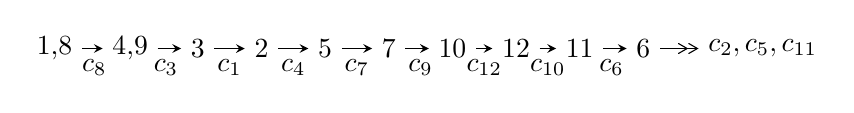
\begin{tikzpicture}[x=23pt, y=7pt]
	% node
	\node (A0) at (-1/8, 0) {1,8};
	\node (A1) at (17/16, 0) {4,9};
	\node (A2) at (17/8, 0) {3};
	\node (A3) at (25/8, 0) {2};
	\node (A4) at (33/8, 0) {5};
	\node (A5) at (41/8, 0) {7};
	\node (A6) at (49/8, 0) {10};
	\node (A7) at (57/8, 0) {12};
	\node (A8) at (65/8, 0) {11};
	\node (A9) at (73/8, 0) {6};
	\node (C1) at (1/2, -1) {$c_{8}$};
	\node (C2) at (13/8, -1) {$c_{3}$};
	\node (C3) at (21/8, -1) {$c_{1}$};
	\node (C4) at (29/8, -1) {$c_{4}$};
	\node (C5) at (37/8, -1) {$c_{7}$};
	\node (C6) at (45/8, -1) {$c_{9}$};
	\node (C7) at (53/8, -1) {$c_{12}$};
	\node (C8) at (61/8, -1) {$c_{10}$};
	\node (C9) at (69/8, -1) {$c_{6}$};
	\node (A10) at (11, 0) {$c_{2},c_{5},c_{11}$};

	% edge
	\draw[->,>=stealth]	
	(A0) edge (A1) (A1) edge (A2) (A2) edge (A3) (A3) edge (A4) (A4) edge (A5) (A5) edge (A6) (A6) edge (A7) (A7) edge (A8) (A8) edge (A9) ;
	\draw[->>,>={angle 60}]	
	(A9) edge (A10);
\end{tikzpicture} \\ 

\end{tabular} \\

\footnotetext{
The image of knot diagram is generated by the software ``\textbf{Draw programme}" developed by Andrew Bartholomew(\url{http://www.layer8.co.uk/maths/draw/index.htm\#Running-draw}), where we modified some parts for our purpose(\url{https://github.com/CATsTAILs/LinksPainter}).
}\phantom \\ \newline 
\centering \textbf{Ideals for irreducible components\footnotemark of $X_{\text{par}}$} 
 
\begin{align*}
I^u_{1}&=\langle 
1.10803\times10^{416} u^{106}-1.09715\times10^{417} u^{105}+\cdots+5.32892\times10^{419} b+1.96754\times10^{419},\\
\phantom{I^u_{1}}&\phantom{= \langle  }3.86181\times10^{419} u^{106}-3.10040\times10^{420} u^{105}+\cdots+2.82433\times10^{421} a+1.15704\times10^{423},\\
\phantom{I^u_{1}}&\phantom{= \langle  }u^{107}-8 u^{106}+\cdots+3774 u-53\rangle \\
I^u_{2}&=\langle 
b,\;- u^3+a- u+1,\;u^4+u^2- u+1\rangle \\
I^u_{3}&=\langle 
b,\;- u^5- u^4-2 u^3-2 u^2+a-2 u-2,\;u^6+u^5+2 u^4+2 u^3+2 u^2+2 u+1\rangle \\
\\
\end{align*}
\raggedright * 3 irreducible components of $\dim_{\mathbb{C}}=0$, with total 117 representations.\\
\footnotetext{All coefficients of polynomials are rational numbers. But the coefficients are sometimes approximated in decimal forms when there is not enough margin.}
\newpage
\renewcommand{\arraystretch}{1}
\centering \section*{I. $I^u_{1}= \langle 1.11\times10^{416} u^{106}-1.10\times10^{417} u^{105}+\cdots+5.33\times10^{419} b+1.97\times10^{419},\;3.86\times10^{419} u^{106}-3.10\times10^{420} u^{105}+\cdots+2.82\times10^{421} a+1.16\times10^{423},\;u^{107}-8 u^{106}+\cdots+3774 u-53 \rangle$}
\flushleft \textbf{(i) Arc colorings}\\
\begin{tabular}{m{7pt} m{180pt} m{7pt} m{180pt} }
\flushright $a_{1}=$&$\begin{pmatrix}0\\u\end{pmatrix}$ \\
\flushright $a_{8}=$&$\begin{pmatrix}1\\0\end{pmatrix}$ \\
\flushright $a_{4}=$&$\begin{pmatrix}-0.0136734 u^{106}+0.109775 u^{105}+\cdots-1.84820 u-40.9669\\-0.000207928 u^{106}+0.00205885 u^{105}+\cdots-14.7641 u-0.369218\end{pmatrix}$ \\
\flushright $a_{9}=$&$\begin{pmatrix}1\\u^2\end{pmatrix}$ \\
\flushright $a_{3}=$&$\begin{pmatrix}-0.0138813 u^{106}+0.111834 u^{105}+\cdots-16.6123 u-41.3361\\-0.000207928 u^{106}+0.00205885 u^{105}+\cdots-14.7641 u-0.369218\end{pmatrix}$ \\
\flushright $a_{2}=$&$\begin{pmatrix}-0.00866897 u^{106}+0.0691354 u^{105}+\cdots+28.1372 u-24.9369\\-0.000596204 u^{106}+0.00486010 u^{105}+\cdots+3.21655 u-0.369377\end{pmatrix}$ \\
\flushright $a_{5}=$&$\begin{pmatrix}-0.00815307 u^{106}+0.0646793 u^{105}+\cdots+32.1684 u-22.5508\\-0.000596204 u^{106}+0.00486010 u^{105}+\cdots+3.21655 u-0.369377\end{pmatrix}$ \\
\flushright $a_{7}=$&$\begin{pmatrix}-0.00642410 u^{106}+0.0508524 u^{105}+\cdots+49.7193 u-22.6538\\-0.000545278 u^{106}+0.00430644 u^{105}+\cdots+8.21892 u-0.432113\end{pmatrix}$ \\
\flushright $a_{10}=$&$\begin{pmatrix}-0.00313420 u^{106}+0.0257724 u^{105}+\cdots-48.1889 u-5.16381\\-0.000447025 u^{106}+0.00376175 u^{105}+\cdots-13.7999 u+0.0889698\end{pmatrix}$ \\
\flushright $a_{12}=$&$\begin{pmatrix}u\\u^3+u\end{pmatrix}$ \\
\flushright $a_{11}=$&$\begin{pmatrix}-0.00309075 u^{106}+0.0255452 u^{105}+\cdots-44.8549 u-5.20870\\-0.000405615 u^{106}+0.00336633 u^{105}+\cdots-10.9176 u+0.0504615\end{pmatrix}$ \\
\flushright $a_{6}=$&$\begin{pmatrix}-0.00211014 u^{106}+0.0160755 u^{105}+\cdots+111.322 u-21.7904\\0.000434043 u^{106}-0.00378194 u^{105}+\cdots+20.5546 u-0.562495\end{pmatrix}$\\&\end{tabular}
\flushleft \textbf{(ii) Obstruction class $= -1$}\\~\\
\flushleft \textbf{(iii) Cusp Shapes $= -0.00735456 u^{106}+0.0589369 u^{105}+\cdots-56.4719 u-8.55387$}\\~\\
\newpage\renewcommand{\arraystretch}{1}
\flushleft \textbf{(iv) u-Polynomials at the component}\newline \\
\begin{tabular}{m{50pt}|m{274pt}}
Crossings & \hspace{64pt}u-Polynomials at each crossing \\
\hline $$\begin{aligned}c_{1}\end{aligned}$$&$\begin{aligned}
&u^{107}+47 u^{106}+\cdots- u+1
\end{aligned}$\\
\hline $$\begin{aligned}c_{2},c_{4}\end{aligned}$$&$\begin{aligned}
&u^{107}-11 u^{106}+\cdots-11 u+1
\end{aligned}$\\
\hline $$\begin{aligned}c_{3},c_{7}\end{aligned}$$&$\begin{aligned}
&u^{107}+u^{106}+\cdots+2048 u+1024
\end{aligned}$\\
\hline $$\begin{aligned}c_{5}\end{aligned}$$&$\begin{aligned}
&u^{107}-2 u^{106}+\cdots+33648 u+4360
\end{aligned}$\\
\hline $$\begin{aligned}c_{6},c_{11}\end{aligned}$$&$\begin{aligned}
&u^{107}+2 u^{106}+\cdots+4 u+1
\end{aligned}$\\
\hline $$\begin{aligned}c_{8},c_{12}\end{aligned}$$&$\begin{aligned}
&u^{107}-8 u^{106}+\cdots+3774 u-53
\end{aligned}$\\
\hline $$\begin{aligned}c_{9}\end{aligned}$$&$\begin{aligned}
&u^{107}+10 u^{106}+\cdots+976 u+64
\end{aligned}$\\
\hline $$\begin{aligned}c_{10}\end{aligned}$$&$\begin{aligned}
&u^{107}-52 u^{106}+\cdots+8 u+1
\end{aligned}$\\
\hline
\end{tabular}\\~\\
\newpage\renewcommand{\arraystretch}{1}
\flushleft \textbf{(v) Riley Polynomials at the component}\newline \\
\begin{tabular}{m{50pt}|m{274pt}}
Crossings & \hspace{64pt}Riley Polynomials at each crossing \\
\hline $$\begin{aligned}c_{1}\end{aligned}$$&$\begin{aligned}
&y^{107}+37 y^{106}+\cdots+155 y-1
\end{aligned}$\\
\hline $$\begin{aligned}c_{2},c_{4}\end{aligned}$$&$\begin{aligned}
&y^{107}-47 y^{106}+\cdots- y-1
\end{aligned}$\\
\hline $$\begin{aligned}c_{3},c_{7}\end{aligned}$$&$\begin{aligned}
&y^{107}+63 y^{106}+\cdots-30932992 y-1048576
\end{aligned}$\\
\hline $$\begin{aligned}c_{5}\end{aligned}$$&$\begin{aligned}
&y^{107}-36 y^{106}+\cdots+1065366544 y-19009600
\end{aligned}$\\
\hline $$\begin{aligned}c_{6},c_{11}\end{aligned}$$&$\begin{aligned}
&y^{107}+52 y^{106}+\cdots+8 y-1
\end{aligned}$\\
\hline $$\begin{aligned}c_{8},c_{12}\end{aligned}$$&$\begin{aligned}
&y^{107}+88 y^{106}+\cdots+13858296 y-2809
\end{aligned}$\\
\hline $$\begin{aligned}c_{9}\end{aligned}$$&$\begin{aligned}
&y^{107}-4 y^{106}+\cdots+53376 y-4096
\end{aligned}$\\
\hline $$\begin{aligned}c_{10}\end{aligned}$$&$\begin{aligned}
&y^{107}+8 y^{106}+\cdots+132 y-1
\end{aligned}$\\
\hline
\end{tabular}\\~\\
\newpage\flushleft \textbf{(vi) Complex Volumes and Cusp Shapes}
$$\begin{array}{c|c|c}  
\text{Solutions to }I^u_{1}& \I (\text{vol} + \sqrt{-1}CS) & \text{Cusp shape}\\
 \hline 
\begin{aligned}
u &= -0.244278 + 0.967291 I \\
a &= \phantom{-}0.15439 + 2.43118 I \\
b &= \phantom{-}0.110417 - 0.860774 I\end{aligned}
 & -1.63198 + 2.05257 I & \phantom{-0.000000 } 0 \\ \hline\begin{aligned}
u &= -0.244278 - 0.967291 I \\
a &= \phantom{-}0.15439 - 2.43118 I \\
b &= \phantom{-}0.110417 + 0.860774 I\end{aligned}
 & -1.63198 - 2.05257 I & \phantom{-0.000000 } 0 \\ \hline\begin{aligned}
u &= \phantom{-}0.717600 + 0.714940 I \\
a &= -0.044492 - 0.756078 I \\
b &= \phantom{-}0.395055 + 0.774024 I\end{aligned}
 & \phantom{-}1.89343 - 6.93711 I & \phantom{-0.000000 } 0 \\ \hline\begin{aligned}
u &= \phantom{-}0.717600 - 0.714940 I \\
a &= -0.044492 + 0.756078 I \\
b &= \phantom{-}0.395055 - 0.774024 I\end{aligned}
 & \phantom{-}1.89343 + 6.93711 I & \phantom{-0.000000 } 0 \\ \hline\begin{aligned}
u &= \phantom{-}0.558306 + 0.801140 I \\
a &= \phantom{-}0.377242 - 0.625630 I \\
b &= \phantom{-}0.138099 + 0.946607 I\end{aligned}
 & \phantom{-}3.73567 + 0.13008 I & \phantom{-0.000000 } 0 \\ \hline\begin{aligned}
u &= \phantom{-}0.558306 - 0.801140 I \\
a &= \phantom{-}0.377242 + 0.625630 I \\
b &= \phantom{-}0.138099 - 0.946607 I\end{aligned}
 & \phantom{-}3.73567 - 0.13008 I & \phantom{-0.000000 } 0 \\ \hline\begin{aligned}
u &= \phantom{-}0.106700 + 0.961946 I \\
a &= \phantom{-}0.067239 + 0.134211 I \\
b &= -0.969199 + 0.200550 I\end{aligned}
 & -0.0780580 + 0.0329782 I & \phantom{-0.000000 } 0 \\ \hline\begin{aligned}
u &= \phantom{-}0.106700 - 0.961946 I \\
a &= \phantom{-}0.067239 - 0.134211 I \\
b &= -0.969199 - 0.200550 I\end{aligned}
 & -0.0780580 - 0.0329782 I & \phantom{-0.000000 } 0 \\ \hline\begin{aligned}
u &= \phantom{-}0.795488 + 0.531373 I \\
a &= -0.818911 + 0.454003 I \\
b &= -0.438711 - 1.131220 I\end{aligned}
 & \phantom{-}2.45043 - 4.63695 I & \phantom{-0.000000 } 0 \\ \hline\begin{aligned}
u &= \phantom{-}0.795488 - 0.531373 I \\
a &= -0.818911 - 0.454003 I \\
b &= -0.438711 + 1.131220 I\end{aligned}
 & \phantom{-}2.45043 + 4.63695 I & \phantom{-0.000000 } 0\\
 \hline 
 \end{array}$$\newpage$$\begin{array}{c|c|c}  
\text{Solutions to }I^u_{1}& \I (\text{vol} + \sqrt{-1}CS) & \text{Cusp shape}\\
 \hline 
\begin{aligned}
u &= \phantom{-}0.378376 + 0.979346 I \\
a &= \phantom{-}0.055561 - 0.405278 I \\
b &= \phantom{-}0.043777 + 0.657390 I\end{aligned}
 & \phantom{-}3.73900 + 0.24041 I & \phantom{-0.000000 } 0 \\ \hline\begin{aligned}
u &= \phantom{-}0.378376 - 0.979346 I \\
a &= \phantom{-}0.055561 + 0.405278 I \\
b &= \phantom{-}0.043777 - 0.657390 I\end{aligned}
 & \phantom{-}3.73900 - 0.24041 I & \phantom{-0.000000 } 0 \\ \hline\begin{aligned}
u &= \phantom{-}0.843285 + 0.392565 I \\
a &= -0.538159 - 0.841495 I \\
b &= -0.767046 + 0.528555 I\end{aligned}
 & -1.74871 - 6.44193 I & \phantom{-0.000000 } 0 \\ \hline\begin{aligned}
u &= \phantom{-}0.843285 - 0.392565 I \\
a &= -0.538159 + 0.841495 I \\
b &= -0.767046 - 0.528555 I\end{aligned}
 & -1.74871 + 6.44193 I & \phantom{-0.000000 } 0 \\ \hline\begin{aligned}
u &= -0.619548 + 0.633428 I \\
a &= \phantom{-}0.069724 - 0.636140 I \\
b &= -0.339848 + 0.674275 I\end{aligned}
 & -0.26443 + 2.25224 I & \phantom{-0.000000 } 0 \\ \hline\begin{aligned}
u &= -0.619548 - 0.633428 I \\
a &= \phantom{-}0.069724 + 0.636140 I \\
b &= -0.339848 - 0.674275 I\end{aligned}
 & -0.26443 - 2.25224 I & \phantom{-0.000000 } 0 \\ \hline\begin{aligned}
u &= \phantom{-}0.824445 + 0.189026 I \\
a &= -0.75491 + 1.63349 I \\
b &= -0.534754 - 0.657037 I\end{aligned}
 & -2.06068 - 4.19793 I & \phantom{-0.000000 } 0 \\ \hline\begin{aligned}
u &= \phantom{-}0.824445 - 0.189026 I \\
a &= -0.75491 - 1.63349 I \\
b &= -0.534754 + 0.657037 I\end{aligned}
 & -2.06068 + 4.19793 I & \phantom{-0.000000 } 0 \\ \hline\begin{aligned}
u &= \phantom{-}1.029330 + 0.531564 I \\
a &= \phantom{-}0.121699 - 0.141240 I \\
b &= -0.206401 + 0.885382 I\end{aligned}
 & -0.39437 + 4.15714 I & \phantom{-0.000000 } 0 \\ \hline\begin{aligned}
u &= \phantom{-}1.029330 - 0.531564 I \\
a &= \phantom{-}0.121699 + 0.141240 I \\
b &= -0.206401 - 0.885382 I\end{aligned}
 & -0.39437 - 4.15714 I & \phantom{-0.000000 } 0\\
 \hline 
 \end{array}$$\newpage$$\begin{array}{c|c|c}  
\text{Solutions to }I^u_{1}& \I (\text{vol} + \sqrt{-1}CS) & \text{Cusp shape}\\
 \hline 
\begin{aligned}
u &= -0.933441 + 0.702521 I \\
a &= -0.183881 - 0.207962 I \\
b &= \phantom{-}0.141803 + 0.854176 I\end{aligned}
 & -1.52785 + 0.45819 I & \phantom{-0.000000 } 0 \\ \hline\begin{aligned}
u &= -0.933441 - 0.702521 I \\
a &= -0.183881 + 0.207962 I \\
b &= \phantom{-}0.141803 - 0.854176 I\end{aligned}
 & -1.52785 - 0.45819 I & \phantom{-0.000000 } 0 \\ \hline\begin{aligned}
u &= -0.782378 + 0.261649 I \\
a &= \phantom{-}0.724726 - 0.937397 I \\
b &= \phantom{-}0.703522 + 0.525334 I\end{aligned}
 & -3.66184 + 1.83985 I & \phantom{-0.000000 } 0 \\ \hline\begin{aligned}
u &= -0.782378 - 0.261649 I \\
a &= \phantom{-}0.724726 + 0.937397 I \\
b &= \phantom{-}0.703522 - 0.525334 I\end{aligned}
 & -3.66184 - 1.83985 I & \phantom{-0.000000 } 0 \\ \hline\begin{aligned}
u &= -1.177060 + 0.290474 I \\
a &= \phantom{-}0.338803 + 0.320303 I \\
b &= \phantom{-}0.430656 - 1.007280 I\end{aligned}
 & -2.48557 + 4.37342 I & \phantom{-0.000000 } 0 \\ \hline\begin{aligned}
u &= -1.177060 - 0.290474 I \\
a &= \phantom{-}0.338803 - 0.320303 I \\
b &= \phantom{-}0.430656 + 1.007280 I\end{aligned}
 & -2.48557 - 4.37342 I & \phantom{-0.000000 } 0 \\ \hline\begin{aligned}
u &= -0.328686 + 1.168570 I \\
a &= -0.148668 - 0.117283 I \\
b &= \phantom{-}1.038800 + 0.287656 I\end{aligned}
 & -0.35619 + 4.34573 I & \phantom{-0.000000 } 0 \\ \hline\begin{aligned}
u &= -0.328686 - 1.168570 I \\
a &= -0.148668 + 0.117283 I \\
b &= \phantom{-}1.038800 - 0.287656 I\end{aligned}
 & -0.35619 - 4.34573 I & \phantom{-0.000000 } 0 \\ \hline\begin{aligned}
u &= \phantom{-}1.221280 + 0.130481 I \\
a &= -0.239161 + 0.249668 I \\
b &= -0.400063 - 0.972833 I\end{aligned}
 & -1.027490 + 0.372205 I & \phantom{-0.000000 } 0 \\ \hline\begin{aligned}
u &= \phantom{-}1.221280 - 0.130481 I \\
a &= -0.239161 - 0.249668 I \\
b &= -0.400063 + 0.972833 I\end{aligned}
 & -1.027490 - 0.372205 I & \phantom{-0.000000 } 0\\
 \hline 
 \end{array}$$\newpage$$\begin{array}{c|c|c}  
\text{Solutions to }I^u_{1}& \I (\text{vol} + \sqrt{-1}CS) & \text{Cusp shape}\\
 \hline 
\begin{aligned}
u &= -0.768164 + 0.030095 I \\
a &= \phantom{-}0.88462 + 1.39992 I \\
b &= \phantom{-}0.578075 - 0.587317 I\end{aligned}
 & -3.83121 - 0.30767 I & -13.13167 + 0. I\phantom{ +0.000000I} \\ \hline\begin{aligned}
u &= -0.768164 - 0.030095 I \\
a &= \phantom{-}0.88462 - 1.39992 I \\
b &= \phantom{-}0.578075 + 0.587317 I\end{aligned}
 & -3.83121 + 0.30767 I & -13.13167 + 0. I\phantom{ +0.000000I} \\ \hline\begin{aligned}
u &= -0.763131 + 0.968657 I \\
a &= -0.156194 - 0.327440 I \\
b &= \phantom{-}0.050991 + 0.764285 I\end{aligned}
 & -0.43303 + 2.32507 I & \phantom{-0.000000 } 0 \\ \hline\begin{aligned}
u &= -0.763131 - 0.968657 I \\
a &= -0.156194 + 0.327440 I \\
b &= \phantom{-}0.050991 - 0.764285 I\end{aligned}
 & -0.43303 - 2.32507 I & \phantom{-0.000000 } 0 \\ \hline\begin{aligned}
u &= -0.091985 + 1.240100 I \\
a &= \phantom{-}0.77646 + 1.78490 I \\
b &= \phantom{-}0.54374 - 1.36147 I\end{aligned}
 & \phantom{-}8.61264 - 0.05840 I & \phantom{-0.000000 } 0 \\ \hline\begin{aligned}
u &= -0.091985 - 1.240100 I \\
a &= \phantom{-}0.77646 - 1.78490 I \\
b &= \phantom{-}0.54374 + 1.36147 I\end{aligned}
 & \phantom{-}8.61264 + 0.05840 I & \phantom{-0.000000 } 0 \\ \hline\begin{aligned}
u &= \phantom{-}0.178080 + 1.246850 I \\
a &= -0.76240 + 1.69178 I \\
b &= -0.55134 - 1.34274 I\end{aligned}
 & \phantom{-}5.90630 - 4.72731 I & \phantom{-0.000000 } 0 \\ \hline\begin{aligned}
u &= \phantom{-}0.178080 - 1.246850 I \\
a &= -0.76240 - 1.69178 I \\
b &= -0.55134 + 1.34274 I\end{aligned}
 & \phantom{-}5.90630 + 4.72731 I & \phantom{-0.000000 } 0 \\ \hline\begin{aligned}
u &= -0.145556 + 1.253260 I \\
a &= \phantom{-}0.364469 + 0.147648 I \\
b &= -1.089070 + 0.127073 I\end{aligned}
 & \phantom{-}1.99962 + 1.17025 I & \phantom{-0.000000 } 0 \\ \hline\begin{aligned}
u &= -0.145556 - 1.253260 I \\
a &= \phantom{-}0.364469 - 0.147648 I \\
b &= -1.089070 - 0.127073 I\end{aligned}
 & \phantom{-}1.99962 - 1.17025 I & \phantom{-0.000000 } 0\\
 \hline 
 \end{array}$$\newpage$$\begin{array}{c|c|c}  
\text{Solutions to }I^u_{1}& \I (\text{vol} + \sqrt{-1}CS) & \text{Cusp shape}\\
 \hline 
\begin{aligned}
u &= -1.135400 + 0.570705 I \\
a &= \phantom{-}0.443382 + 0.526000 I \\
b &= \phantom{-}0.489972 - 1.055080 I\end{aligned}
 & -1.97155 + 6.45339 I & \phantom{-0.000000 } 0 \\ \hline\begin{aligned}
u &= -1.135400 - 0.570705 I \\
a &= \phantom{-}0.443382 - 0.526000 I \\
b &= \phantom{-}0.489972 + 1.055080 I\end{aligned}
 & -1.97155 - 6.45339 I & \phantom{-0.000000 } 0 \\ \hline\begin{aligned}
u &= \phantom{-}0.468996 + 0.530095 I \\
a &= -0.68912 + 2.39644 I \\
b &= -0.280440 - 0.684314 I\end{aligned}
 & -0.98884 + 1.84483 I & -3.82797 + 1.28640 I \\ \hline\begin{aligned}
u &= \phantom{-}0.468996 - 0.530095 I \\
a &= -0.68912 - 2.39644 I \\
b &= -0.280440 + 0.684314 I\end{aligned}
 & -0.98884 - 1.84483 I & -3.82797 - 1.28640 I \\ \hline\begin{aligned}
u &= \phantom{-}0.405837 + 0.572578 I \\
a &= -0.570749 - 0.083950 I \\
b &= -0.802591 + 0.320828 I\end{aligned}
 & -0.174410 - 0.127515 I & -5.50445 + 1.13479 I \\ \hline\begin{aligned}
u &= \phantom{-}0.405837 - 0.572578 I \\
a &= -0.570749 + 0.083950 I \\
b &= -0.802591 - 0.320828 I\end{aligned}
 & -0.174410 + 0.127515 I & -5.50445 - 1.13479 I \\ \hline\begin{aligned}
u &= -0.291545 + 1.287990 I \\
a &= \phantom{-}0.07916 + 2.30407 I \\
b &= \phantom{-}0.110803 - 0.993595 I\end{aligned}
 & \phantom{-}0.23928 + 3.46090 I & \phantom{-0.000000 } 0 \\ \hline\begin{aligned}
u &= -0.291545 - 1.287990 I \\
a &= \phantom{-}0.07916 - 2.30407 I \\
b &= \phantom{-}0.110803 + 0.993595 I\end{aligned}
 & \phantom{-}0.23928 - 3.46090 I & \phantom{-0.000000 } 0 \\ \hline\begin{aligned}
u &= \phantom{-}0.209184 + 1.304430 I \\
a &= -0.412576 + 0.156149 I \\
b &= \phantom{-}1.111000 + 0.109634 I\end{aligned}
 & \phantom{-}4.56308 - 6.01047 I & \phantom{-0.000000 } 0 \\ \hline\begin{aligned}
u &= \phantom{-}0.209184 - 1.304430 I \\
a &= -0.412576 - 0.156149 I \\
b &= \phantom{-}1.111000 - 0.109634 I\end{aligned}
 & \phantom{-}4.56308 + 6.01047 I & \phantom{-0.000000 } 0\\
 \hline 
 \end{array}$$\newpage$$\begin{array}{c|c|c}  
\text{Solutions to }I^u_{1}& \I (\text{vol} + \sqrt{-1}CS) & \text{Cusp shape}\\
 \hline 
\begin{aligned}
u &= \phantom{-}0.265083 + 1.299270 I \\
a &= \phantom{-}0.42759 - 1.54289 I \\
b &= \phantom{-}0.327691 + 1.304980 I\end{aligned}
 & \phantom{-}4.98675 + 0.12143 I & \phantom{-0.000000 } 0 \\ \hline\begin{aligned}
u &= \phantom{-}0.265083 - 1.299270 I \\
a &= \phantom{-}0.42759 + 1.54289 I \\
b &= \phantom{-}0.327691 - 1.304980 I\end{aligned}
 & \phantom{-}4.98675 - 0.12143 I & \phantom{-0.000000 } 0 \\ \hline\begin{aligned}
u &= \phantom{-}0.744053 + 1.104860 I \\
a &= \phantom{-}0.118395 - 0.327376 I \\
b &= -0.054853 + 0.717685 I\end{aligned}
 & \phantom{-}1.82231 - 7.19731 I & \phantom{-0.000000 } 0 \\ \hline\begin{aligned}
u &= \phantom{-}0.744053 - 1.104860 I \\
a &= \phantom{-}0.118395 + 0.327376 I \\
b &= -0.054853 - 0.717685 I\end{aligned}
 & \phantom{-}1.82231 + 7.19731 I & \phantom{-0.000000 } 0 \\ \hline\begin{aligned}
u &= \phantom{-}1.149480 + 0.694236 I \\
a &= -0.434365 + 0.627438 I \\
b &= -0.519863 - 1.067400 I\end{aligned}
 & -0.01179 - 11.33370 I & \phantom{-0.000000 } 0 \\ \hline\begin{aligned}
u &= \phantom{-}1.149480 - 0.694236 I \\
a &= -0.434365 - 0.627438 I \\
b &= -0.519863 + 1.067400 I\end{aligned}
 & -0.01179 + 11.33370 I & \phantom{-0.000000 } 0 \\ \hline\begin{aligned}
u &= \phantom{-}0.067332 + 1.356370 I \\
a &= -0.385316 + 0.071591 I \\
b &= \phantom{-}1.118240 + 0.160068 I\end{aligned}
 & \phantom{-}6.21427 + 2.01067 I & \phantom{-0.000000 } 0 \\ \hline\begin{aligned}
u &= \phantom{-}0.067332 - 1.356370 I \\
a &= -0.385316 - 0.071591 I \\
b &= \phantom{-}1.118240 - 0.160068 I\end{aligned}
 & \phantom{-}6.21427 - 2.01067 I & \phantom{-0.000000 } 0 \\ \hline\begin{aligned}
u &= \phantom{-}0.043841 + 1.358030 I \\
a &= \phantom{-}0.49776 - 1.75459 I \\
b &= \phantom{-}0.29145 + 1.39069 I\end{aligned}
 & \phantom{-}7.49723 + 1.30975 I & \phantom{-0.000000 } 0 \\ \hline\begin{aligned}
u &= \phantom{-}0.043841 - 1.358030 I \\
a &= \phantom{-}0.49776 + 1.75459 I \\
b &= \phantom{-}0.29145 - 1.39069 I\end{aligned}
 & \phantom{-}7.49723 - 1.30975 I & \phantom{-0.000000 } 0\\
 \hline 
 \end{array}$$\newpage$$\begin{array}{c|c|c}  
\text{Solutions to }I^u_{1}& \I (\text{vol} + \sqrt{-1}CS) & \text{Cusp shape}\\
 \hline 
\begin{aligned}
u &= \phantom{-}0.016598 + 1.368280 I \\
a &= -0.51049 - 1.80982 I \\
b &= -0.28157 + 1.41137 I\end{aligned}
 & \phantom{-}10.15850 - 6.16266 I & \phantom{-0.000000 } 0 \\ \hline\begin{aligned}
u &= \phantom{-}0.016598 - 1.368280 I \\
a &= -0.51049 + 1.80982 I \\
b &= -0.28157 - 1.41137 I\end{aligned}
 & \phantom{-}10.15850 + 6.16266 I & \phantom{-0.000000 } 0 \\ \hline\begin{aligned}
u &= \phantom{-}0.177576 + 1.358930 I \\
a &= -0.04241 + 2.30582 I \\
b &= -0.065693 - 1.015390 I\end{aligned}
 & \phantom{-}4.51674 - 0.36965 I & \phantom{-0.000000 } 0 \\ \hline\begin{aligned}
u &= \phantom{-}0.177576 - 1.358930 I \\
a &= -0.04241 - 2.30582 I \\
b &= -0.065693 + 1.015390 I\end{aligned}
 & \phantom{-}4.51674 + 0.36965 I & \phantom{-0.000000 } 0 \\ \hline\begin{aligned}
u &= \phantom{-}0.500396 + 1.282940 I \\
a &= -0.62879 + 1.39268 I \\
b &= -0.584855 - 1.274260 I\end{aligned}
 & \phantom{-}3.20733 - 5.65218 I & \phantom{-0.000000 } 0 \\ \hline\begin{aligned}
u &= \phantom{-}0.500396 - 1.282940 I \\
a &= -0.62879 - 1.39268 I \\
b &= -0.584855 + 1.274260 I\end{aligned}
 & \phantom{-}3.20733 + 5.65218 I & \phantom{-0.000000 } 0 \\ \hline\begin{aligned}
u &= -0.170784 + 1.367340 I \\
a &= \phantom{-}0.64277 + 1.71294 I \\
b &= \phantom{-}0.57737 - 1.35306 I\end{aligned}
 & \phantom{-}10.04680 + 8.11877 I & \phantom{-0.000000 } 0 \\ \hline\begin{aligned}
u &= -0.170784 - 1.367340 I \\
a &= \phantom{-}0.64277 - 1.71294 I \\
b &= \phantom{-}0.57737 + 1.35306 I\end{aligned}
 & \phantom{-}10.04680 - 8.11877 I & \phantom{-0.000000 } 0 \\ \hline\begin{aligned}
u &= \phantom{-}0.331508 + 1.355170 I \\
a &= -0.07380 + 2.28294 I \\
b &= -0.121993 - 1.020340 I\end{aligned}
 & \phantom{-}2.75081 - 8.34322 I & \phantom{-0.000000 } 0 \\ \hline\begin{aligned}
u &= \phantom{-}0.331508 - 1.355170 I \\
a &= -0.07380 - 2.28294 I \\
b &= -0.121993 + 1.020340 I\end{aligned}
 & \phantom{-}2.75081 + 8.34322 I & \phantom{-0.000000 } 0\\
 \hline 
 \end{array}$$\newpage$$\begin{array}{c|c|c}  
\text{Solutions to }I^u_{1}& \I (\text{vol} + \sqrt{-1}CS) & \text{Cusp shape}\\
 \hline 
\begin{aligned}
u &= \phantom{-}0.599443 + 0.047851 I \\
a &= -0.467004 - 0.519575 I \\
b &= \phantom{-}0.580248 + 0.294112 I\end{aligned}
 & \phantom{-}0.59909 + 3.23248 I & -3.54970 - 2.02366 I \\ \hline\begin{aligned}
u &= \phantom{-}0.599443 - 0.047851 I \\
a &= -0.467004 + 0.519575 I \\
b &= \phantom{-}0.580248 - 0.294112 I\end{aligned}
 & \phantom{-}0.59909 - 3.23248 I & -3.54970 + 2.02366 I \\ \hline\begin{aligned}
u &= -0.523910 + 0.283236 I \\
a &= \phantom{-}0.283886 - 0.479371 I \\
b &= -0.413442 + 0.397977 I\end{aligned}
 & -1.003830 + 0.947083 I & -6.72670 - 4.41292 I \\ \hline\begin{aligned}
u &= -0.523910 - 0.283236 I \\
a &= \phantom{-}0.283886 + 0.479371 I \\
b &= -0.413442 - 0.397977 I\end{aligned}
 & -1.003830 - 0.947083 I & -6.72670 + 4.41292 I \\ \hline\begin{aligned}
u &= -0.33909 + 1.40174 I \\
a &= -0.31003 - 1.55968 I \\
b &= -0.381510 + 1.311700 I\end{aligned}
 & \phantom{-}4.72927 + 4.53808 I & \phantom{-0.000000 } 0 \\ \hline\begin{aligned}
u &= -0.33909 - 1.40174 I \\
a &= -0.31003 + 1.55968 I \\
b &= -0.381510 - 1.311700 I\end{aligned}
 & \phantom{-}4.72927 - 4.53808 I & \phantom{-0.000000 } 0 \\ \hline\begin{aligned}
u &= -0.34118 + 1.40161 I \\
a &= -0.304334 - 0.170972 I \\
b &= \phantom{-}1.117030 + 0.295556 I\end{aligned}
 & \phantom{-}1.60903 + 5.96407 I & \phantom{-0.000000 } 0 \\ \hline\begin{aligned}
u &= -0.34118 - 1.40161 I \\
a &= -0.304334 + 0.170972 I \\
b &= \phantom{-}1.117030 - 0.295556 I\end{aligned}
 & \phantom{-}1.60903 - 5.96407 I & \phantom{-0.000000 } 0 \\ \hline\begin{aligned}
u &= -0.06354 + 1.44683 I \\
a &= -0.41932 - 1.77311 I \\
b &= -0.32247 + 1.40483 I\end{aligned}
 & \phantom{-}11.73440 + 2.01740 I & \phantom{-0.000000 } 0 \\ \hline\begin{aligned}
u &= -0.06354 - 1.44683 I \\
a &= -0.41932 + 1.77311 I \\
b &= -0.32247 - 1.40483 I\end{aligned}
 & \phantom{-}11.73440 - 2.01740 I & \phantom{-0.000000 } 0\\
 \hline 
 \end{array}$$\newpage$$\begin{array}{c|c|c}  
\text{Solutions to }I^u_{1}& \I (\text{vol} + \sqrt{-1}CS) & \text{Cusp shape}\\
 \hline 
\begin{aligned}
u &= \phantom{-}0.23844 + 1.43773 I \\
a &= \phantom{-}0.345146 - 0.116560 I \\
b &= -1.131050 + 0.263267 I\end{aligned}
 & \phantom{-}5.97945 - 2.87063 I & \phantom{-0.000000 } 0 \\ \hline\begin{aligned}
u &= \phantom{-}0.23844 - 1.43773 I \\
a &= \phantom{-}0.345146 + 0.116560 I \\
b &= -1.131050 - 0.263267 I\end{aligned}
 & \phantom{-}5.97945 + 2.87063 I & \phantom{-0.000000 } 0 \\ \hline\begin{aligned}
u &= \phantom{-}0.36411 + 1.45966 I \\
a &= \phantom{-}0.335672 - 0.193945 I \\
b &= -1.135240 + 0.303887 I\end{aligned}
 & \phantom{-}4.12324 - 10.89930 I & \phantom{-0.000000 } 0 \\ \hline\begin{aligned}
u &= \phantom{-}0.36411 - 1.45966 I \\
a &= \phantom{-}0.335672 + 0.193945 I \\
b &= -1.135240 - 0.303887 I\end{aligned}
 & \phantom{-}4.12324 + 10.89930 I & \phantom{-0.000000 } 0 \\ \hline\begin{aligned}
u &= \phantom{-}0.355328 + 0.327509 I \\
a &= -0.535333 + 0.829714 I \\
b &= \phantom{-}0.741715 - 0.054497 I\end{aligned}
 & \phantom{-}0.97038 + 3.14809 I & -2.61784 - 5.19860 I \\ \hline\begin{aligned}
u &= \phantom{-}0.355328 - 0.327509 I \\
a &= -0.535333 - 0.829714 I \\
b &= \phantom{-}0.741715 + 0.054497 I\end{aligned}
 & \phantom{-}0.97038 - 3.14809 I & -2.61784 + 5.19860 I \\ \hline\begin{aligned}
u &= -0.52030 + 1.42675 I \\
a &= \phantom{-}0.50897 + 1.43324 I \\
b &= \phantom{-}0.61769 - 1.28222 I\end{aligned}
 & \phantom{-}2.79707 + 10.37630 I & \phantom{-0.000000 } 0 \\ \hline\begin{aligned}
u &= -0.52030 - 1.42675 I \\
a &= \phantom{-}0.50897 - 1.43324 I \\
b &= \phantom{-}0.61769 + 1.28222 I\end{aligned}
 & \phantom{-}2.79707 - 10.37630 I & \phantom{-0.000000 } 0 \\ \hline\begin{aligned}
u &= \phantom{-}0.385481 + 0.157711 I \\
a &= \phantom{-}0.57690 + 1.52323 I \\
b &= -0.191599 + 1.167350 I\end{aligned}
 & \phantom{-}2.53797 + 2.54179 I & -2.10720 - 3.38961 I \\ \hline\begin{aligned}
u &= \phantom{-}0.385481 - 0.157711 I \\
a &= \phantom{-}0.57690 - 1.52323 I \\
b &= -0.191599 - 1.167350 I\end{aligned}
 & \phantom{-}2.53797 - 2.54179 I & -2.10720 + 3.38961 I\\
 \hline 
 \end{array}$$\newpage$$\begin{array}{c|c|c}  
\text{Solutions to }I^u_{1}& \I (\text{vol} + \sqrt{-1}CS) & \text{Cusp shape}\\
 \hline 
\begin{aligned}
u &= \phantom{-}0.26127 + 1.56618 I \\
a &= \phantom{-}0.25567 - 1.69472 I \\
b &= \phantom{-}0.40497 + 1.37995 I\end{aligned}
 & \phantom{-}11.33560 - 3.17947 I & \phantom{-0.000000 } 0 \\ \hline\begin{aligned}
u &= \phantom{-}0.26127 - 1.56618 I \\
a &= \phantom{-}0.25567 + 1.69472 I \\
b &= \phantom{-}0.40497 - 1.37995 I\end{aligned}
 & \phantom{-}11.33560 + 3.17947 I & \phantom{-0.000000 } 0 \\ \hline\begin{aligned}
u &= -0.33545 + 1.55553 I \\
a &= -0.22516 - 1.64887 I \\
b &= -0.42278 + 1.35777 I\end{aligned}
 & \phantom{-}6.87012 + 6.32881 I & \phantom{-0.000000 } 0 \\ \hline\begin{aligned}
u &= -0.33545 - 1.55553 I \\
a &= -0.22516 + 1.64887 I \\
b &= -0.42278 - 1.35777 I\end{aligned}
 & \phantom{-}6.87012 - 6.32881 I & \phantom{-0.000000 } 0 \\ \hline\begin{aligned}
u &= -0.191098 + 0.331866 I \\
a &= -2.48353 + 0.52436 I \\
b &= \phantom{-}0.110517 + 1.223940 I\end{aligned}
 & \phantom{-}5.65239 + 1.11140 I & \phantom{-}2.39761 - 0.78708 I \\ \hline\begin{aligned}
u &= -0.191098 - 0.331866 I \\
a &= -2.48353 - 0.52436 I \\
b &= \phantom{-}0.110517 - 1.223940 I\end{aligned}
 & \phantom{-}5.65239 - 1.11140 I & \phantom{-}2.39761 + 0.78708 I \\ \hline\begin{aligned}
u &= \phantom{-}0.37243 + 1.57605 I \\
a &= -0.44058 + 1.58113 I \\
b &= -0.63720 - 1.32574 I\end{aligned}
 & \phantom{-}9.36952 - 9.23755 I & \phantom{-0.000000 } 0 \\ \hline\begin{aligned}
u &= \phantom{-}0.37243 - 1.57605 I \\
a &= -0.44058 - 1.58113 I \\
b &= -0.63720 + 1.32574 I\end{aligned}
 & \phantom{-}9.36952 + 9.23755 I & \phantom{-0.000000 } 0 \\ \hline\begin{aligned}
u &= \phantom{-}0.34589 + 1.59767 I \\
a &= \phantom{-}0.19820 - 1.66460 I \\
b &= \phantom{-}0.43639 + 1.36713 I\end{aligned}
 & \phantom{-}9.4139 - 11.3192 I & \phantom{-0.000000 } 0 \\ \hline\begin{aligned}
u &= \phantom{-}0.34589 - 1.59767 I \\
a &= \phantom{-}0.19820 + 1.66460 I \\
b &= \phantom{-}0.43639 - 1.36713 I\end{aligned}
 & \phantom{-}9.4139 + 11.3192 I & \phantom{-0.000000 } 0\\
 \hline 
 \end{array}$$\newpage$$\begin{array}{c|c|c}  
\text{Solutions to }I^u_{1}& \I (\text{vol} + \sqrt{-1}CS) & \text{Cusp shape}\\
 \hline 
\begin{aligned}
u &= -0.46077 + 1.59233 I \\
a &= \phantom{-}0.40978 + 1.52343 I \\
b &= \phantom{-}0.64769 - 1.30858 I\end{aligned}
 & \phantom{-}4.83717 + 12.32680 I & \phantom{-0.000000 } 0 \\ \hline\begin{aligned}
u &= -0.46077 - 1.59233 I \\
a &= \phantom{-}0.40978 - 1.52343 I \\
b &= \phantom{-}0.64769 + 1.30858 I\end{aligned}
 & \phantom{-}4.83717 - 12.32680 I & \phantom{-0.000000 } 0 \\ \hline\begin{aligned}
u &= \phantom{-}0.45699 + 1.64231 I \\
a &= -0.37754 + 1.53751 I \\
b &= -0.65776 - 1.31344 I\end{aligned}
 & \phantom{-}7.3438 - 17.3524 I & \phantom{-0.000000 } 0 \\ \hline\begin{aligned}
u &= \phantom{-}0.45699 - 1.64231 I \\
a &= -0.37754 - 1.53751 I \\
b &= -0.65776 + 1.31344 I\end{aligned}
 & \phantom{-}7.3438 + 17.3524 I & \phantom{-0.000000 } 0 \\ \hline\begin{aligned}
u &= -0.192027 + 0.008415 I \\
a &= \phantom{-}0.89307 + 5.19596 I \\
b &= \phantom{-}0.224018 + 1.245620 I\end{aligned}
 & \phantom{-}5.41652 - 6.50120 I & \phantom{-}1.62481 + 7.00024 I \\ \hline\begin{aligned}
u &= -0.192027 - 0.008415 I \\
a &= \phantom{-}0.89307 - 5.19596 I \\
b &= \phantom{-}0.224018 - 1.245620 I\end{aligned}
 & \phantom{-}5.41652 + 6.50120 I & \phantom{-}1.62481 - 7.00024 I \\ \hline\begin{aligned}
u &= \phantom{-}0.0143062\phantom{ +0.000000I} \\
a &= -40.7428\phantom{ +0.000000I} \\
b &= -0.560782\phantom{ +0.000000I}\end{aligned}
 & -1.12189\phantom{ +0.000000I} & -9.23230\phantom{ +0.000000I}\\
 \hline 
 \end{array}$$\newpage\newpage\renewcommand{\arraystretch}{1}
\centering \section*{II. $I^u_{2}= \langle b,\;- u^3+a- u+1,\;u^4+u^2- u+1 \rangle$}
\flushleft \textbf{(i) Arc colorings}\\
\begin{tabular}{m{7pt} m{180pt} m{7pt} m{180pt} }
\flushright $a_{1}=$&$\begin{pmatrix}0\\u\end{pmatrix}$ \\
\flushright $a_{8}=$&$\begin{pmatrix}1\\0\end{pmatrix}$ \\
\flushright $a_{4}=$&$\begin{pmatrix}u^3+u-1\\0\end{pmatrix}$ \\
\flushright $a_{9}=$&$\begin{pmatrix}1\\u^2\end{pmatrix}$ \\
\flushright $a_{3}=$&$\begin{pmatrix}u^3+u-1\\0\end{pmatrix}$ \\
\flushright $a_{2}=$&$\begin{pmatrix}u^3+u-1\\u\end{pmatrix}$ \\
\flushright $a_{5}=$&$\begin{pmatrix}0\\- u\end{pmatrix}$ \\
\flushright $a_{7}=$&$\begin{pmatrix}1\\0\end{pmatrix}$ \\
\flushright $a_{10}=$&$\begin{pmatrix}u^2+1\\u^2\end{pmatrix}$ \\
\flushright $a_{12}=$&$\begin{pmatrix}u\\u^3+u\end{pmatrix}$ \\
\flushright $a_{11}=$&$\begin{pmatrix}- u^3+u^2+1\\u\end{pmatrix}$ \\
\flushright $a_{6}=$&$\begin{pmatrix}- u^3- u^2\\- u^2\end{pmatrix}$\\&\end{tabular}
\flushleft \textbf{(ii) Obstruction class $= 1$}\\~\\
\flushleft \textbf{(iii) Cusp Shapes $= 3 u^3+4 u^2- u-10$}\\~\\
\newpage\renewcommand{\arraystretch}{1}
\flushleft \textbf{(iv) u-Polynomials at the component}\newline \\
\begin{tabular}{m{50pt}|m{274pt}}
Crossings & \hspace{64pt}u-Polynomials at each crossing \\
\hline $$\begin{aligned}c_{1},c_{2}\end{aligned}$$&$\begin{aligned}
&(u-1)^4
\end{aligned}$\\
\hline $$\begin{aligned}c_{3},c_{7}\end{aligned}$$&$\begin{aligned}
&u^4
\end{aligned}$\\
\hline $$\begin{aligned}c_{4}\end{aligned}$$&$\begin{aligned}
&(u+1)^4
\end{aligned}$\\
\hline $$\begin{aligned}c_{5}\end{aligned}$$&$\begin{aligned}
&u^4-3 u^3+4 u^2-3 u+2
\end{aligned}$\\
\hline $$\begin{aligned}c_{6},c_{8}\end{aligned}$$&$\begin{aligned}
&u^4+u^2- u+1
\end{aligned}$\\
\hline $$\begin{aligned}c_{9}\end{aligned}$$&$\begin{aligned}
&u^4-2 u^3+3 u^2- u+1
\end{aligned}$\\
\hline $$\begin{aligned}c_{10}\end{aligned}$$&$\begin{aligned}
&u^4+2 u^3+3 u^2+u+1
\end{aligned}$\\
\hline $$\begin{aligned}c_{11},c_{12}\end{aligned}$$&$\begin{aligned}
&u^4+u^2+u+1
\end{aligned}$\\
\hline
\end{tabular}\\~\\
\newpage\renewcommand{\arraystretch}{1}
\flushleft \textbf{(v) Riley Polynomials at the component}\newline \\
\begin{tabular}{m{50pt}|m{274pt}}
Crossings & \hspace{64pt}Riley Polynomials at each crossing \\
\hline $$\begin{aligned}c_{1},c_{2},c_{4}\end{aligned}$$&$\begin{aligned}
&(y-1)^4
\end{aligned}$\\
\hline $$\begin{aligned}c_{3},c_{7}\end{aligned}$$&$\begin{aligned}
&y^4
\end{aligned}$\\
\hline $$\begin{aligned}c_{5}\end{aligned}$$&$\begin{aligned}
&y^4- y^3+2 y^2+7 y+4
\end{aligned}$\\
\hline $$\begin{aligned}c_{6},c_{8},c_{11}\\c_{12}\end{aligned}$$&$\begin{aligned}
&y^4+2 y^3+3 y^2+y+1
\end{aligned}$\\
\hline $$\begin{aligned}c_{9},c_{10}\end{aligned}$$&$\begin{aligned}
&y^4+2 y^3+7 y^2+5 y+1
\end{aligned}$\\
\hline
\end{tabular}\\~\\
\newpage\flushleft \textbf{(vi) Complex Volumes and Cusp Shapes}
$$\begin{array}{c|c|c}  
\text{Solutions to }I^u_{2}& \I (\text{vol} + \sqrt{-1}CS) & \text{Cusp shape}\\
 \hline 
\begin{aligned}
u &= \phantom{-}0.547424 + 0.585652 I \\
a &= -0.851808 + 0.911292 I \\
b &= \phantom{-0.000000 } 0\end{aligned}
 & -2.62503 - 1.39709 I & -11.91838 + 2.95607 I \\ \hline\begin{aligned}
u &= \phantom{-}0.547424 - 0.585652 I \\
a &= -0.851808 - 0.911292 I \\
b &= \phantom{-0.000000 } 0\end{aligned}
 & -2.62503 + 1.39709 I & -11.91838 - 2.95607 I \\ \hline\begin{aligned}
u &= -0.547424 + 1.120870 I \\
a &= \phantom{-}0.351808 + 0.720342 I \\
b &= \phantom{-0.000000 } 0\end{aligned}
 & \phantom{-}0.98010 + 7.64338 I & -7.58162 - 7.23121 I \\ \hline\begin{aligned}
u &= -0.547424 - 1.120870 I \\
a &= \phantom{-}0.351808 - 0.720342 I \\
b &= \phantom{-0.000000 } 0\end{aligned}
 & \phantom{-}0.98010 - 7.64338 I & -7.58162 + 7.23121 I\\
 \hline 
 \end{array}$$\newpage\newpage\renewcommand{\arraystretch}{1}
\centering \section*{III. $I^u_{3}= \langle b,\;- u^5- u^4-2 u^3-2 u^2+a-2 u-2,\;u^6+u^5+2 u^4+2 u^3+2 u^2+2 u+1 \rangle$}
\flushleft \textbf{(i) Arc colorings}\\
\begin{tabular}{m{7pt} m{180pt} m{7pt} m{180pt} }
\flushright $a_{1}=$&$\begin{pmatrix}0\\u\end{pmatrix}$ \\
\flushright $a_{8}=$&$\begin{pmatrix}1\\0\end{pmatrix}$ \\
\flushright $a_{4}=$&$\begin{pmatrix}u^5+u^4+2 u^3+2 u^2+2 u+2\\0\end{pmatrix}$ \\
\flushright $a_{9}=$&$\begin{pmatrix}1\\u^2\end{pmatrix}$ \\
\flushright $a_{3}=$&$\begin{pmatrix}u^5+u^4+2 u^3+2 u^2+2 u+2\\0\end{pmatrix}$ \\
\flushright $a_{2}=$&$\begin{pmatrix}u^5+u^4+2 u^3+2 u^2+2 u+2\\u\end{pmatrix}$ \\
\flushright $a_{5}=$&$\begin{pmatrix}0\\- u\end{pmatrix}$ \\
\flushright $a_{7}=$&$\begin{pmatrix}1\\0\end{pmatrix}$ \\
\flushright $a_{10}=$&$\begin{pmatrix}u^2+1\\u^2\end{pmatrix}$ \\
\flushright $a_{12}=$&$\begin{pmatrix}u\\u^3+u\end{pmatrix}$ \\
\flushright $a_{11}=$&$\begin{pmatrix}u^5+u^4+2 u^3+2 u^2+2 u+2\\u^5+2 u^3+u^2+u+1\end{pmatrix}$ \\
\flushright $a_{6}=$&$\begin{pmatrix}- u^5-2 u^3- u\\- u^5- u^3- u\end{pmatrix}$\\&\end{tabular}
\flushleft \textbf{(ii) Obstruction class $= 1$}\\~\\
\flushleft \textbf{(iii) Cusp Shapes $= 2 u^5+u^4+7 u^3+3 u^2+6 u-4$}\\~\\
\newpage\renewcommand{\arraystretch}{1}
\flushleft \textbf{(iv) u-Polynomials at the component}\newline \\
\begin{tabular}{m{50pt}|m{274pt}}
Crossings & \hspace{64pt}u-Polynomials at each crossing \\
\hline $$\begin{aligned}c_{1},c_{2}\end{aligned}$$&$\begin{aligned}
&(u-1)^6
\end{aligned}$\\
\hline $$\begin{aligned}c_{3},c_{7}\end{aligned}$$&$\begin{aligned}
&u^6
\end{aligned}$\\
\hline $$\begin{aligned}c_{4}\end{aligned}$$&$\begin{aligned}
&(u+1)^6
\end{aligned}$\\
\hline $$\begin{aligned}c_{5}\end{aligned}$$&$\begin{aligned}
&(u^3+u^2-1)^2
\end{aligned}$\\
\hline $$\begin{aligned}c_{6},c_{8}\end{aligned}$$&$\begin{aligned}
&u^6+u^5+2 u^4+2 u^3+2 u^2+2 u+1
\end{aligned}$\\
\hline $$\begin{aligned}c_{9}\end{aligned}$$&$\begin{aligned}
&u^6-3 u^5+4 u^4-2 u^3+1
\end{aligned}$\\
\hline $$\begin{aligned}c_{10}\end{aligned}$$&$\begin{aligned}
&u^6+3 u^5+4 u^4+2 u^3+1
\end{aligned}$\\
\hline $$\begin{aligned}c_{11},c_{12}\end{aligned}$$&$\begin{aligned}
&u^6- u^5+2 u^4-2 u^3+2 u^2-2 u+1
\end{aligned}$\\
\hline
\end{tabular}\\~\\
\newpage\renewcommand{\arraystretch}{1}
\flushleft \textbf{(v) Riley Polynomials at the component}\newline \\
\begin{tabular}{m{50pt}|m{274pt}}
Crossings & \hspace{64pt}Riley Polynomials at each crossing \\
\hline $$\begin{aligned}c_{1},c_{2},c_{4}\end{aligned}$$&$\begin{aligned}
&(y-1)^6
\end{aligned}$\\
\hline $$\begin{aligned}c_{3},c_{7}\end{aligned}$$&$\begin{aligned}
&y^6
\end{aligned}$\\
\hline $$\begin{aligned}c_{5}\end{aligned}$$&$\begin{aligned}
&(y^3- y^2+2 y-1)^2
\end{aligned}$\\
\hline $$\begin{aligned}c_{6},c_{8},c_{11}\\c_{12}\end{aligned}$$&$\begin{aligned}
&y^6+3 y^5+4 y^4+2 y^3+1
\end{aligned}$\\
\hline $$\begin{aligned}c_{9},c_{10}\end{aligned}$$&$\begin{aligned}
&y^6- y^5+4 y^4-2 y^3+8 y^2+1
\end{aligned}$\\
\hline
\end{tabular}\\~\\
\newpage\flushleft \textbf{(vi) Complex Volumes and Cusp Shapes}
$$\begin{array}{c|c|c}  
\text{Solutions to }I^u_{3}& \I (\text{vol} + \sqrt{-1}CS) & \text{Cusp shape}\\
 \hline 
\begin{aligned}
u &= \phantom{-}0.498832 + 1.001300 I \\
a &= -0.398606 + 0.800120 I \\
b &= \phantom{-0.000000 } 0\end{aligned}
 & -1.37919 - 2.82812 I & -10.74483 + 3.34054 I \\ \hline\begin{aligned}
u &= \phantom{-}0.498832 - 1.001300 I \\
a &= -0.398606 - 0.800120 I \\
b &= \phantom{-0.000000 } 0\end{aligned}
 & -1.37919 + 2.82812 I & -10.74483 - 3.34054 I \\ \hline\begin{aligned}
u &= -0.284920 + 1.115140 I \\
a &= \phantom{-}0.215080 + 0.841795 I \\
b &= \phantom{-0.000000 } 0\end{aligned}
 & \phantom{-}2.75839\phantom{ +0.000000I} & -4.80521 - 0.27335 I \\ \hline\begin{aligned}
u &= -0.284920 - 1.115140 I \\
a &= \phantom{-}0.215080 - 0.841795 I \\
b &= \phantom{-0.000000 } 0\end{aligned}
 & \phantom{-}2.75839\phantom{ +0.000000I} & -4.80521 + 0.27335 I \\ \hline\begin{aligned}
u &= -0.713912 + 0.305839 I \\
a &= \phantom{-}1.183530 + 0.507021 I \\
b &= \phantom{-0.000000 } 0\end{aligned}
 & -1.37919 - 2.82812 I & -7.94996 + 3.74291 I \\ \hline\begin{aligned}
u &= -0.713912 - 0.305839 I \\
a &= \phantom{-}1.183530 - 0.507021 I \\
b &= \phantom{-0.000000 } 0\end{aligned}
 & -1.37919 + 2.82812 I & -7.94996 - 3.74291 I\\
 \hline 
 \end{array}$$\newpage
\newpage\renewcommand{\arraystretch}{1}
\centering \section*{ IV. u-Polynomials}
\begin{tabular}{m{50pt}|m{274pt}}
Crossings & \hspace{64pt}u-Polynomials at each crossing \\
\hline $$\begin{aligned}c_{1}\end{aligned}$$&$\begin{aligned}
&((u-1)^{10})(u^{107}+47 u^{106}+\cdots- u+1)
\end{aligned}$\\
\hline $$\begin{aligned}c_{2}\end{aligned}$$&$\begin{aligned}
&((u-1)^{10})(u^{107}-11 u^{106}+\cdots-11 u+1)
\end{aligned}$\\
\hline $$\begin{aligned}c_{3},c_{7}\end{aligned}$$&$\begin{aligned}
&u^{10}(u^{107}+u^{106}+\cdots+2048 u+1024)
\end{aligned}$\\
\hline $$\begin{aligned}c_{4}\end{aligned}$$&$\begin{aligned}
&((u+1)^{10})(u^{107}-11 u^{106}+\cdots-11 u+1)
\end{aligned}$\\
\hline $$\begin{aligned}c_{5}\end{aligned}$$&$\begin{aligned}
&(u^3+u^2-1)^2(u^4-3 u^3+4 u^2-3 u+2)\\
&\cdot(u^{107}-2 u^{106}+\cdots+33648 u+4360)
\end{aligned}$\\
\hline $$\begin{aligned}c_{6}\end{aligned}$$&$\begin{aligned}
&(u^4+u^2- u+1)(u^6+u^5+2 u^4+2 u^3+2 u^2+2 u+1)\\
&\cdot(u^{107}+2 u^{106}+\cdots+4 u+1)
\end{aligned}$\\
\hline $$\begin{aligned}c_{8}\end{aligned}$$&$\begin{aligned}
&(u^4+u^2- u+1)(u^6+u^5+2 u^4+2 u^3+2 u^2+2 u+1)\\
&\cdot(u^{107}-8 u^{106}+\cdots+3774 u-53)
\end{aligned}$\\
\hline $$\begin{aligned}c_{9}\end{aligned}$$&$\begin{aligned}
&(u^4-2 u^3+3 u^2- u+1)(u^6-3 u^5+4 u^4-2 u^3+1)\\
&\cdot(u^{107}+10 u^{106}+\cdots+976 u+64)
\end{aligned}$\\
\hline $$\begin{aligned}c_{10}\end{aligned}$$&$\begin{aligned}
&(u^4+2 u^3+3 u^2+u+1)(u^6+3 u^5+4 u^4+2 u^3+1)\\
&\cdot(u^{107}-52 u^{106}+\cdots+8 u+1)
\end{aligned}$\\
\hline $$\begin{aligned}c_{11}\end{aligned}$$&$\begin{aligned}
&(u^4+u^2+u+1)(u^6- u^5+2 u^4-2 u^3+2 u^2-2 u+1)\\
&\cdot(u^{107}+2 u^{106}+\cdots+4 u+1)
\end{aligned}$\\
\hline $$\begin{aligned}c_{12}\end{aligned}$$&$\begin{aligned}
&(u^4+u^2+u+1)(u^6- u^5+2 u^4-2 u^3+2 u^2-2 u+1)\\
&\cdot(u^{107}-8 u^{106}+\cdots+3774 u-53)
\end{aligned}$\\
\hline
\end{tabular}\newpage\renewcommand{\arraystretch}{1}
\centering \section*{ V. Riley Polynomials}
\begin{tabular}{m{50pt}|m{274pt}}
Crossings & \hspace{64pt}Riley Polynomials at each crossing \\
\hline $$\begin{aligned}c_{1}\end{aligned}$$&$\begin{aligned}
&((y-1)^{10})(y^{107}+37 y^{106}+\cdots+155 y-1)
\end{aligned}$\\
\hline $$\begin{aligned}c_{2},c_{4}\end{aligned}$$&$\begin{aligned}
&((y-1)^{10})(y^{107}-47 y^{106}+\cdots- y-1)
\end{aligned}$\\
\hline $$\begin{aligned}c_{3},c_{7}\end{aligned}$$&$\begin{aligned}
&y^{10}(y^{107}+63 y^{106}+\cdots-3.09330\times10^{7} y-1048576)
\end{aligned}$\\
\hline $$\begin{aligned}c_{5}\end{aligned}$$&$\begin{aligned}
&(y^3- y^2+2 y-1)^2(y^4- y^3+2 y^2+7 y+4)\\
&\cdot(y^{107}-36 y^{106}+\cdots+1065366544 y-19009600)
\end{aligned}$\\
\hline $$\begin{aligned}c_{6},c_{11}\end{aligned}$$&$\begin{aligned}
&(y^4+2 y^3+3 y^2+y+1)(y^6+3 y^5+4 y^4+2 y^3+1)\\
&\cdot(y^{107}+52 y^{106}+\cdots+8 y-1)
\end{aligned}$\\
\hline $$\begin{aligned}c_{8},c_{12}\end{aligned}$$&$\begin{aligned}
&(y^4+2 y^3+3 y^2+y+1)(y^6+3 y^5+4 y^4+2 y^3+1)\\
&\cdot(y^{107}+88 y^{106}+\cdots+13858296 y-2809)
\end{aligned}$\\
\hline $$\begin{aligned}c_{9}\end{aligned}$$&$\begin{aligned}
&(y^4+2 y^3+7 y^2+5 y+1)(y^6- y^5+4 y^4-2 y^3+8 y^2+1)\\
&\cdot(y^{107}-4 y^{106}+\cdots+53376 y-4096)
\end{aligned}$\\
\hline $$\begin{aligned}c_{10}\end{aligned}$$&$\begin{aligned}
&(y^4+2 y^3+7 y^2+5 y+1)(y^6- y^5+4 y^4-2 y^3+8 y^2+1)\\
&\cdot(y^{107}+8 y^{106}+\cdots+132 y-1)
\end{aligned}$\\
\hline
\end{tabular}
\vskip 2pc
\end{document}